% !TEX root = main2.tex
\section{Model and DLV factor visualizations}

\subsection{Consistent Drift}
\label{app:drift}

Figure~\ref{fig:numerics-best-paths} illustrates the fitted measure change
using four matched Model~D paths.  Solid and dashed paths of the same colour
use identical Gaussian draws under $\Q$ and $\PP$.
Solid and dashed lines of the same colour use
the same Gaussian draws under~$\Q$ and~$\PP$.  Besides spot, the illustration
reports ATM one- and five-day implied volatility and the central log-strike skew
\begin{equation}\label{eq:numerics-atm-skew}
  \operatorname{Skew}_{\tau}
  =\frac{
    \sigma_{\mathrm{imp}}(K=Z_t e^h,\tau)
    -\sigma_{\mathrm{imp}}(K=Z_t e^{-h},\tau)
  }{2h},
  \qquad h=0.01.
\end{equation}
The paths illustrate the fitted measure change; four paths are not a physical
model validation.

\begin{figure}[H]
  \centering
  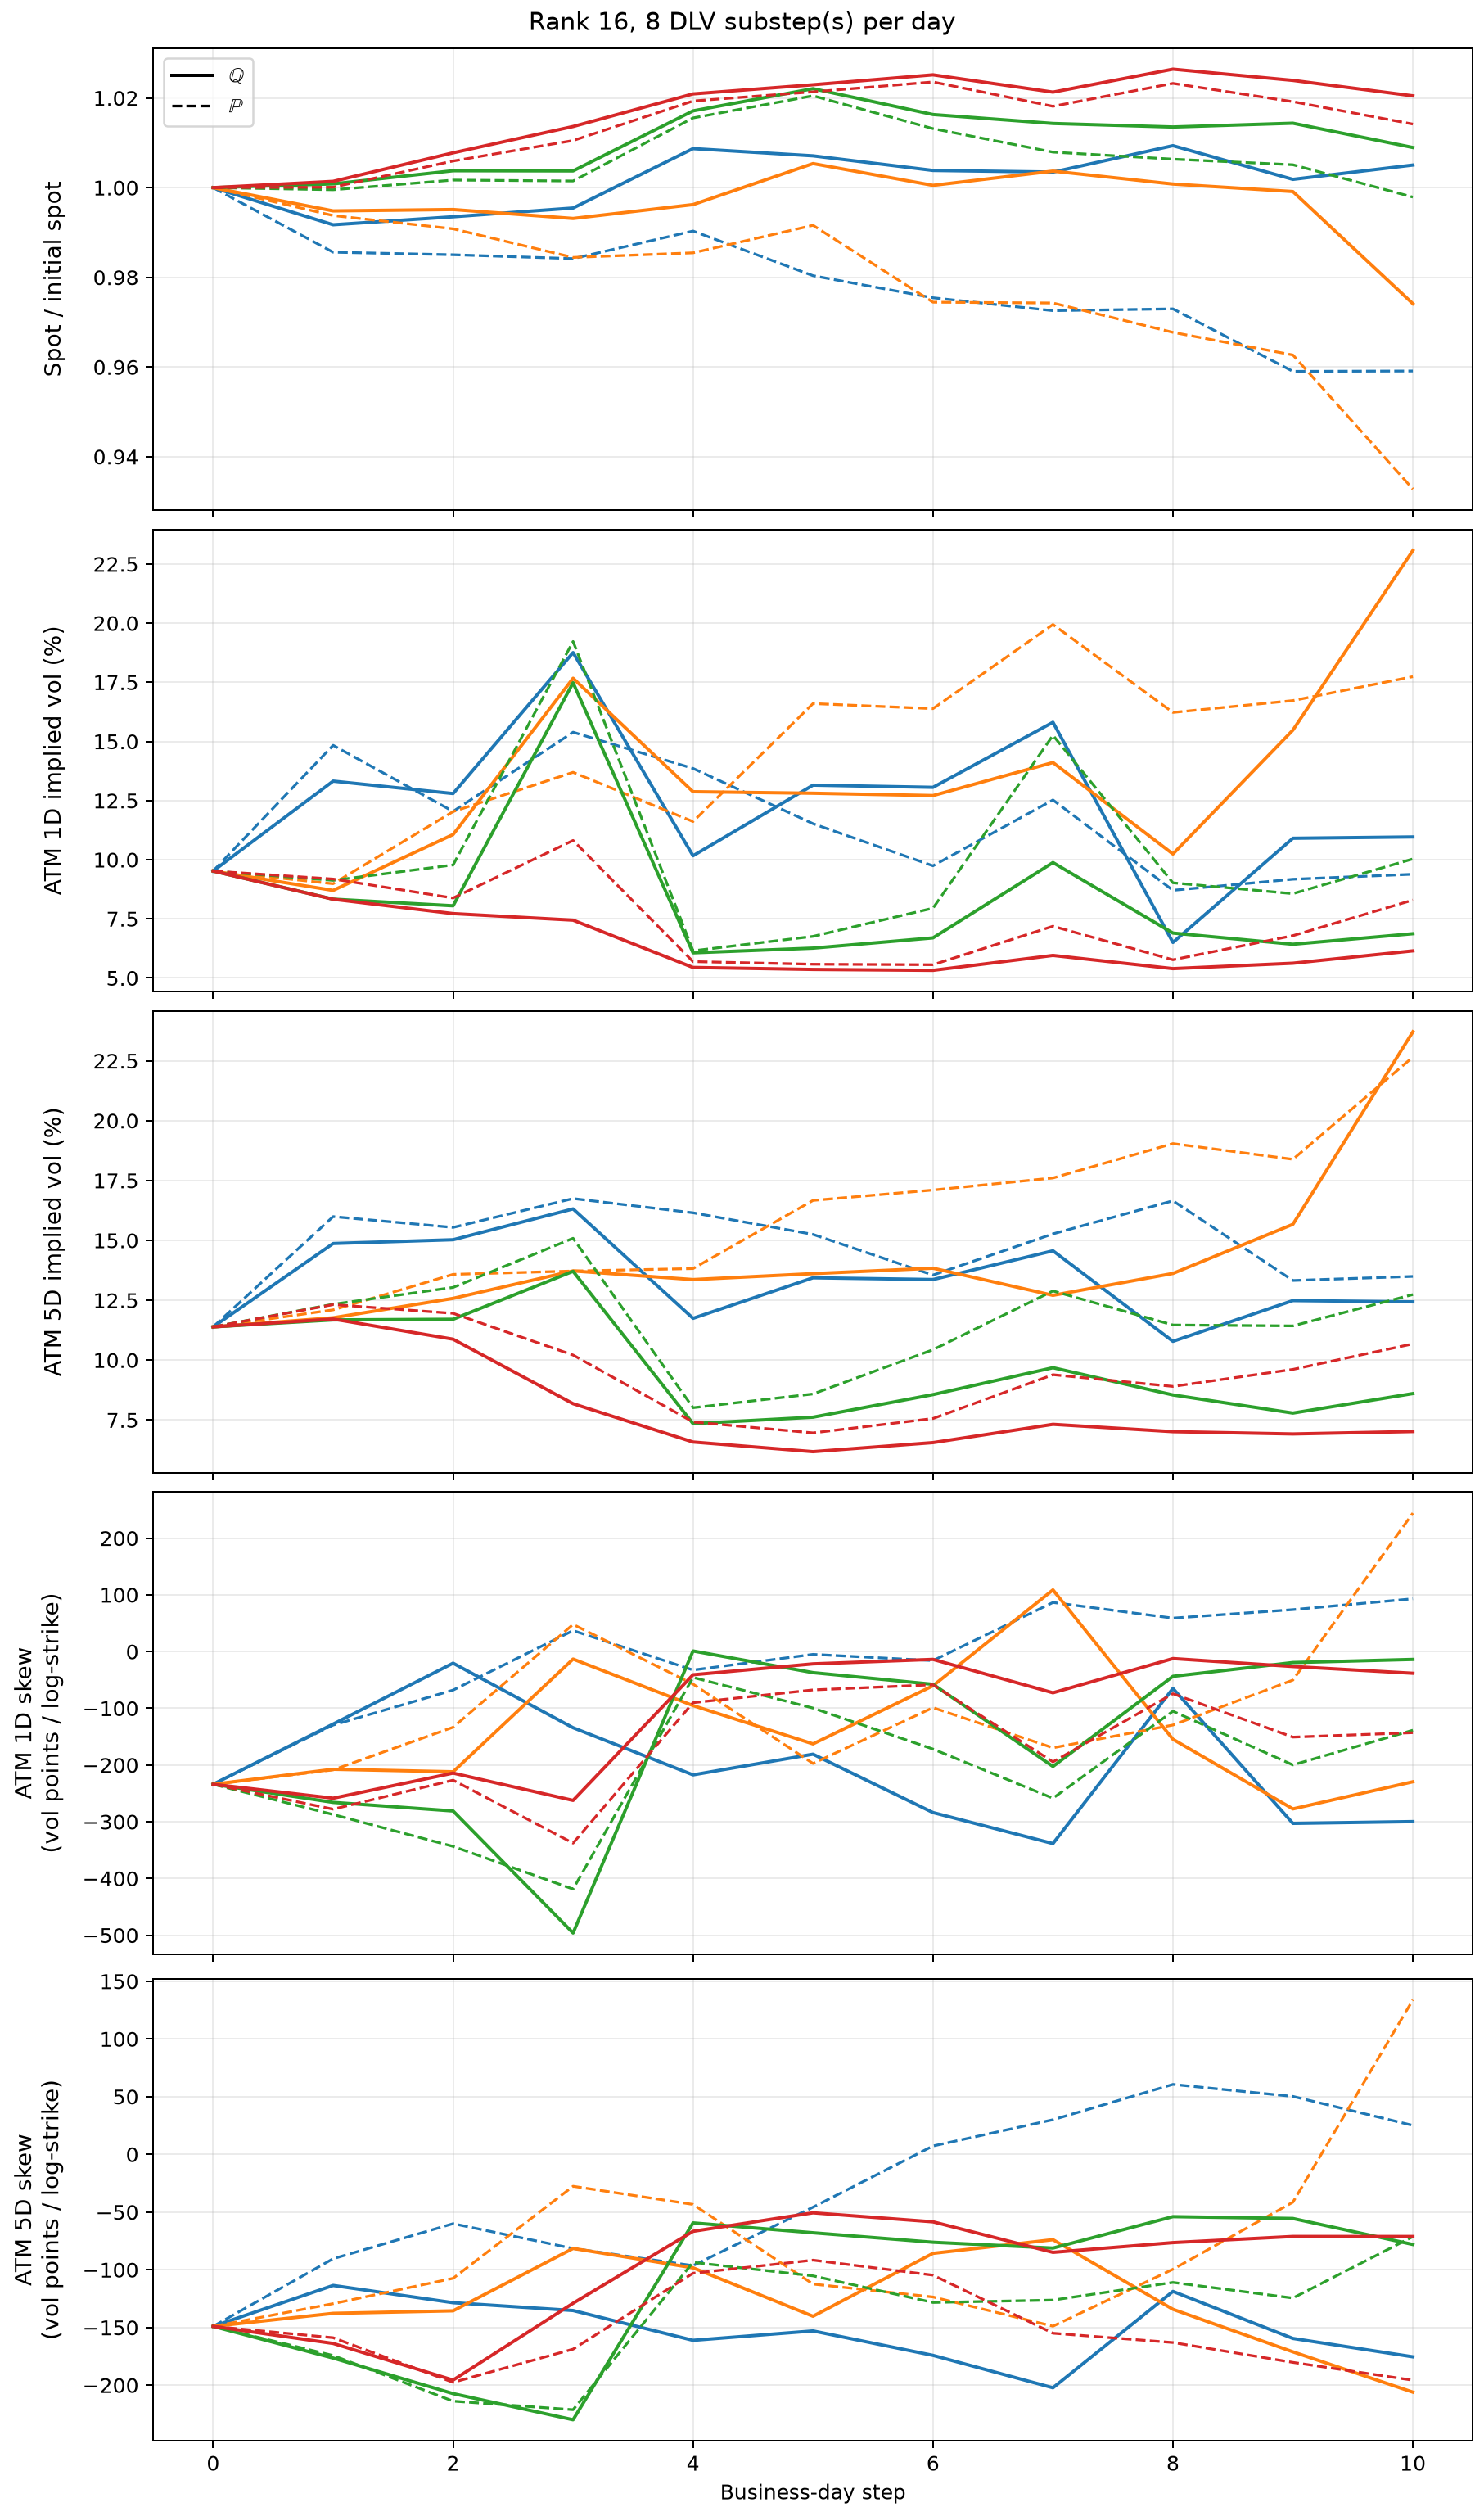
\includegraphics[height=0.88\textheight]
    {figures/front_spot/paths_rank16_eight_step.png}
  \caption{Matched $\PP/\Q$ paths for Model~D: rank 16 with eight Brownian
  substeps per day.}
  \label{fig:numerics-best-paths}
\end{figure}

\subsection{PCA Summary}
\label{app:dlv-factor-figures}

The remaining figures visualize the factor systems estimated in
Section~\ref{sec:estimation-vol-of-vol}.  Figure~\ref{fig:numerics-baseline-iv-3d}
is the baseline risk-neutral implied-volatility surface used for all factor
illustrations.


\begin{figure}[H]
  \centering
  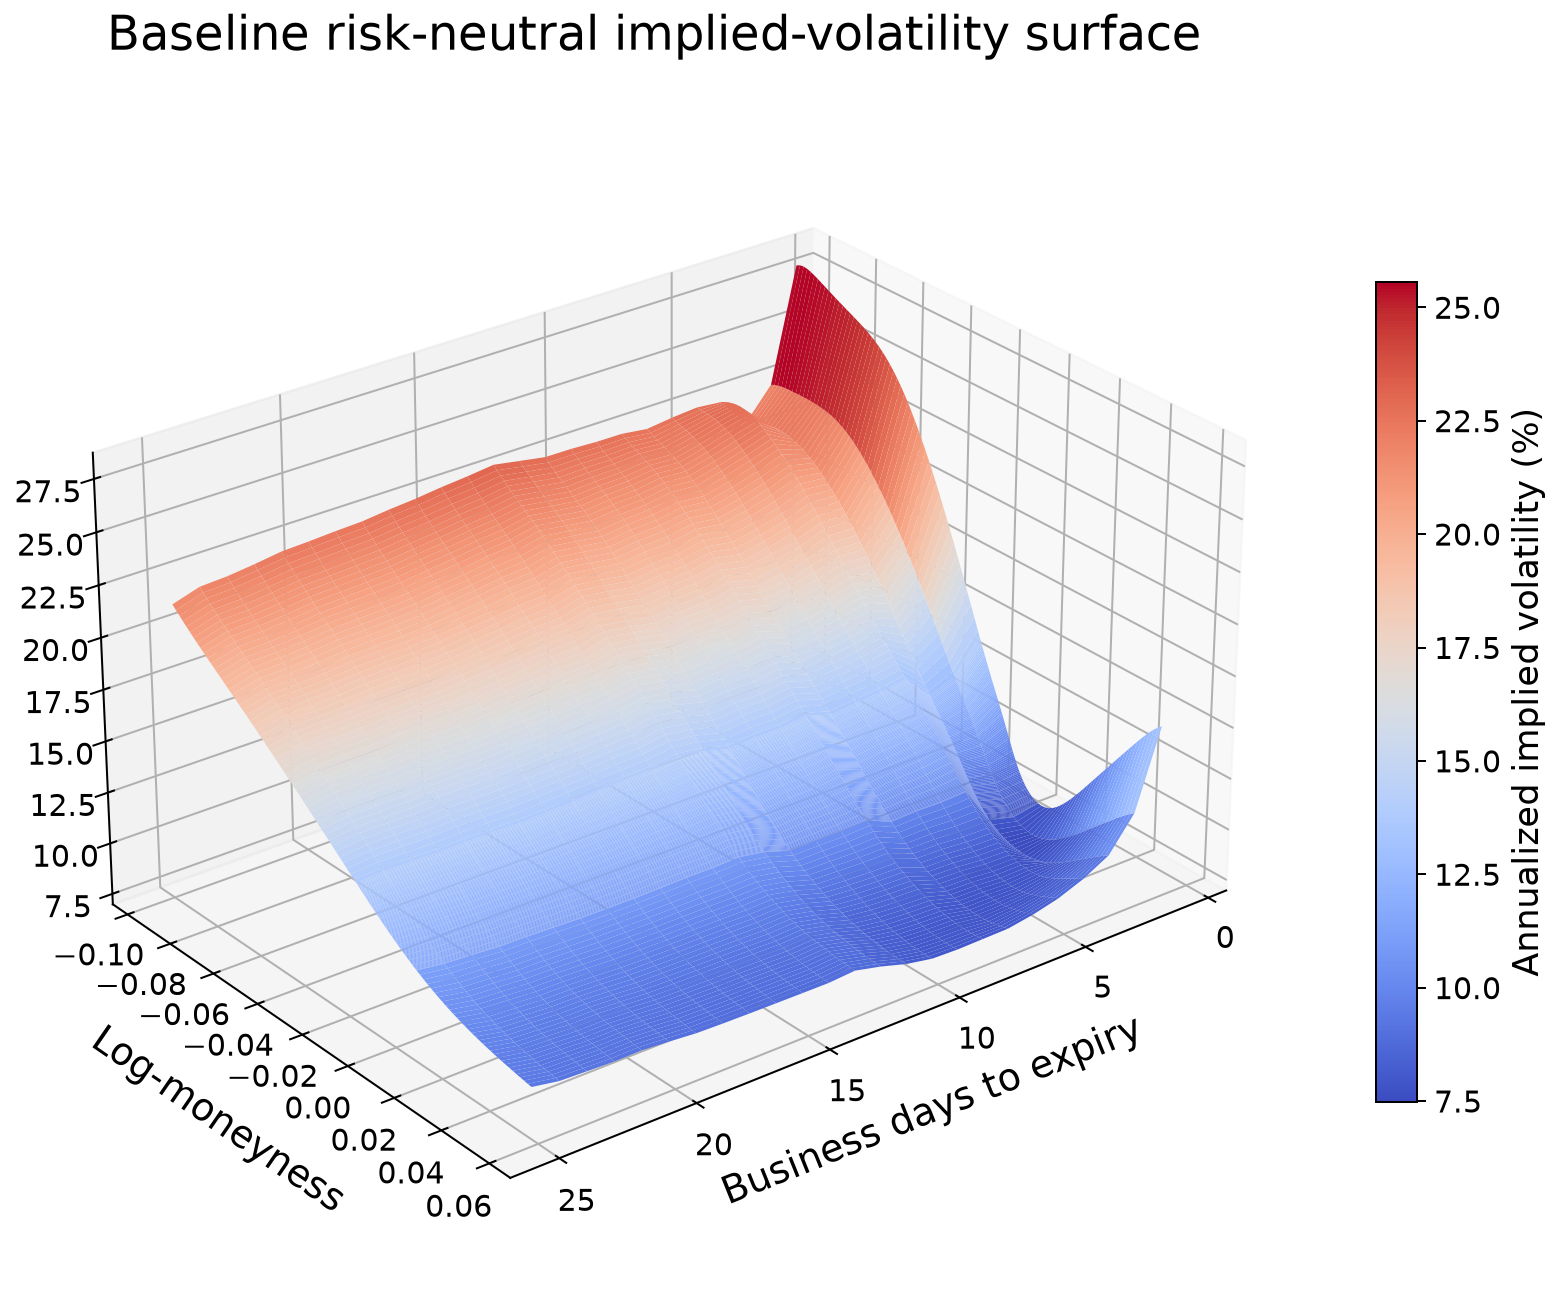
\includegraphics[width=0.72\textwidth]
    {figures/front_spot/baseline_implied_volatility_3d.png}
  \caption{Baseline annualized implied volatility on the fitted
  log-moneyness and business-days-to-expiry grid.}
  \label{fig:numerics-baseline-iv-3d}
\end{figure}

Figure~\ref{fig:numerics-factor-power} reports individual and cumulative PCA
power.  The experiments retain either eight or 16 factors; the first rank
above 90\% is 26.

\begin{figure}[H]
  \centering
  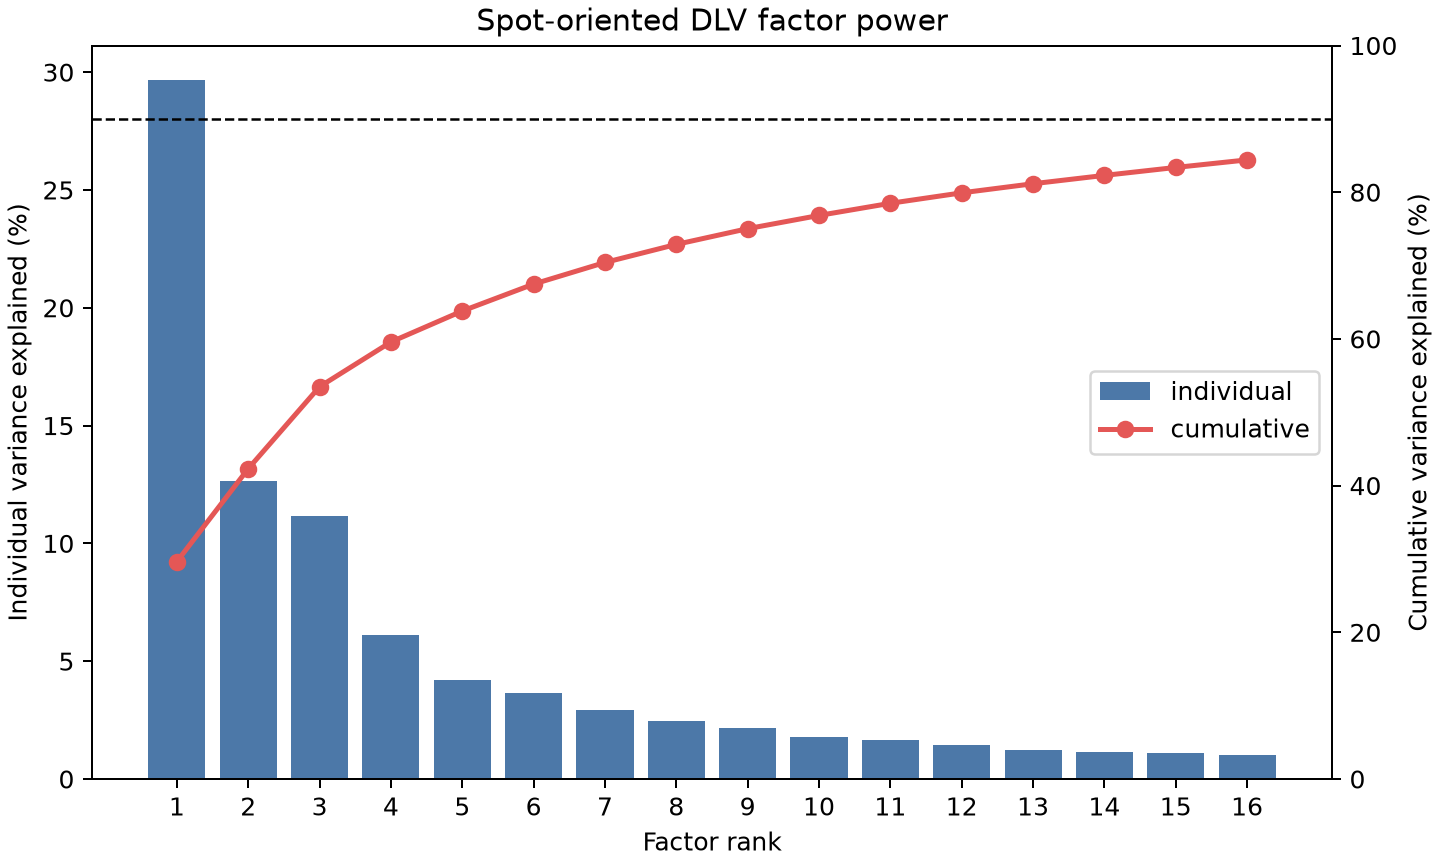
\includegraphics[width=0.88\textwidth]
    {figures/front_spot/pca_explained_variance.png}
  \caption{Individual and cumulative variance explained by the spot-oriented
  DLV factor system.  The vertical line is the rank-16 model cap; 26 factors
  are required to exceed 90\%.}
  \label{fig:numerics-factor-power}
\end{figure}

The rank-16 fit appends PCs 9--16 to the rank-8 fit.  A one-standard-deviation
shock is the diffusion-only log-DLV displacement
$\pm\xi_f\sqrt{1/252}$.  The figures display its central implied-volatility
response
\begin{equation}
  \label{eq:numerics-iv-factor-shock}
  \frac12\left[
    \sigma_{\mathrm{imp}}(\log\Sigma+\xi_f/\sqrt{252})
    -\sigma_{\mathrm{imp}}(\log\Sigma-\xi_f/\sqrt{252})
  \right].
\end{equation}
These shock directions are the same under $\PP$ and $\Q$: an equivalent
measure change alters drift, not diffusion.  Each panel deliberately retains
its own vertical scale.

\begin{figure}[H]
  \centering
  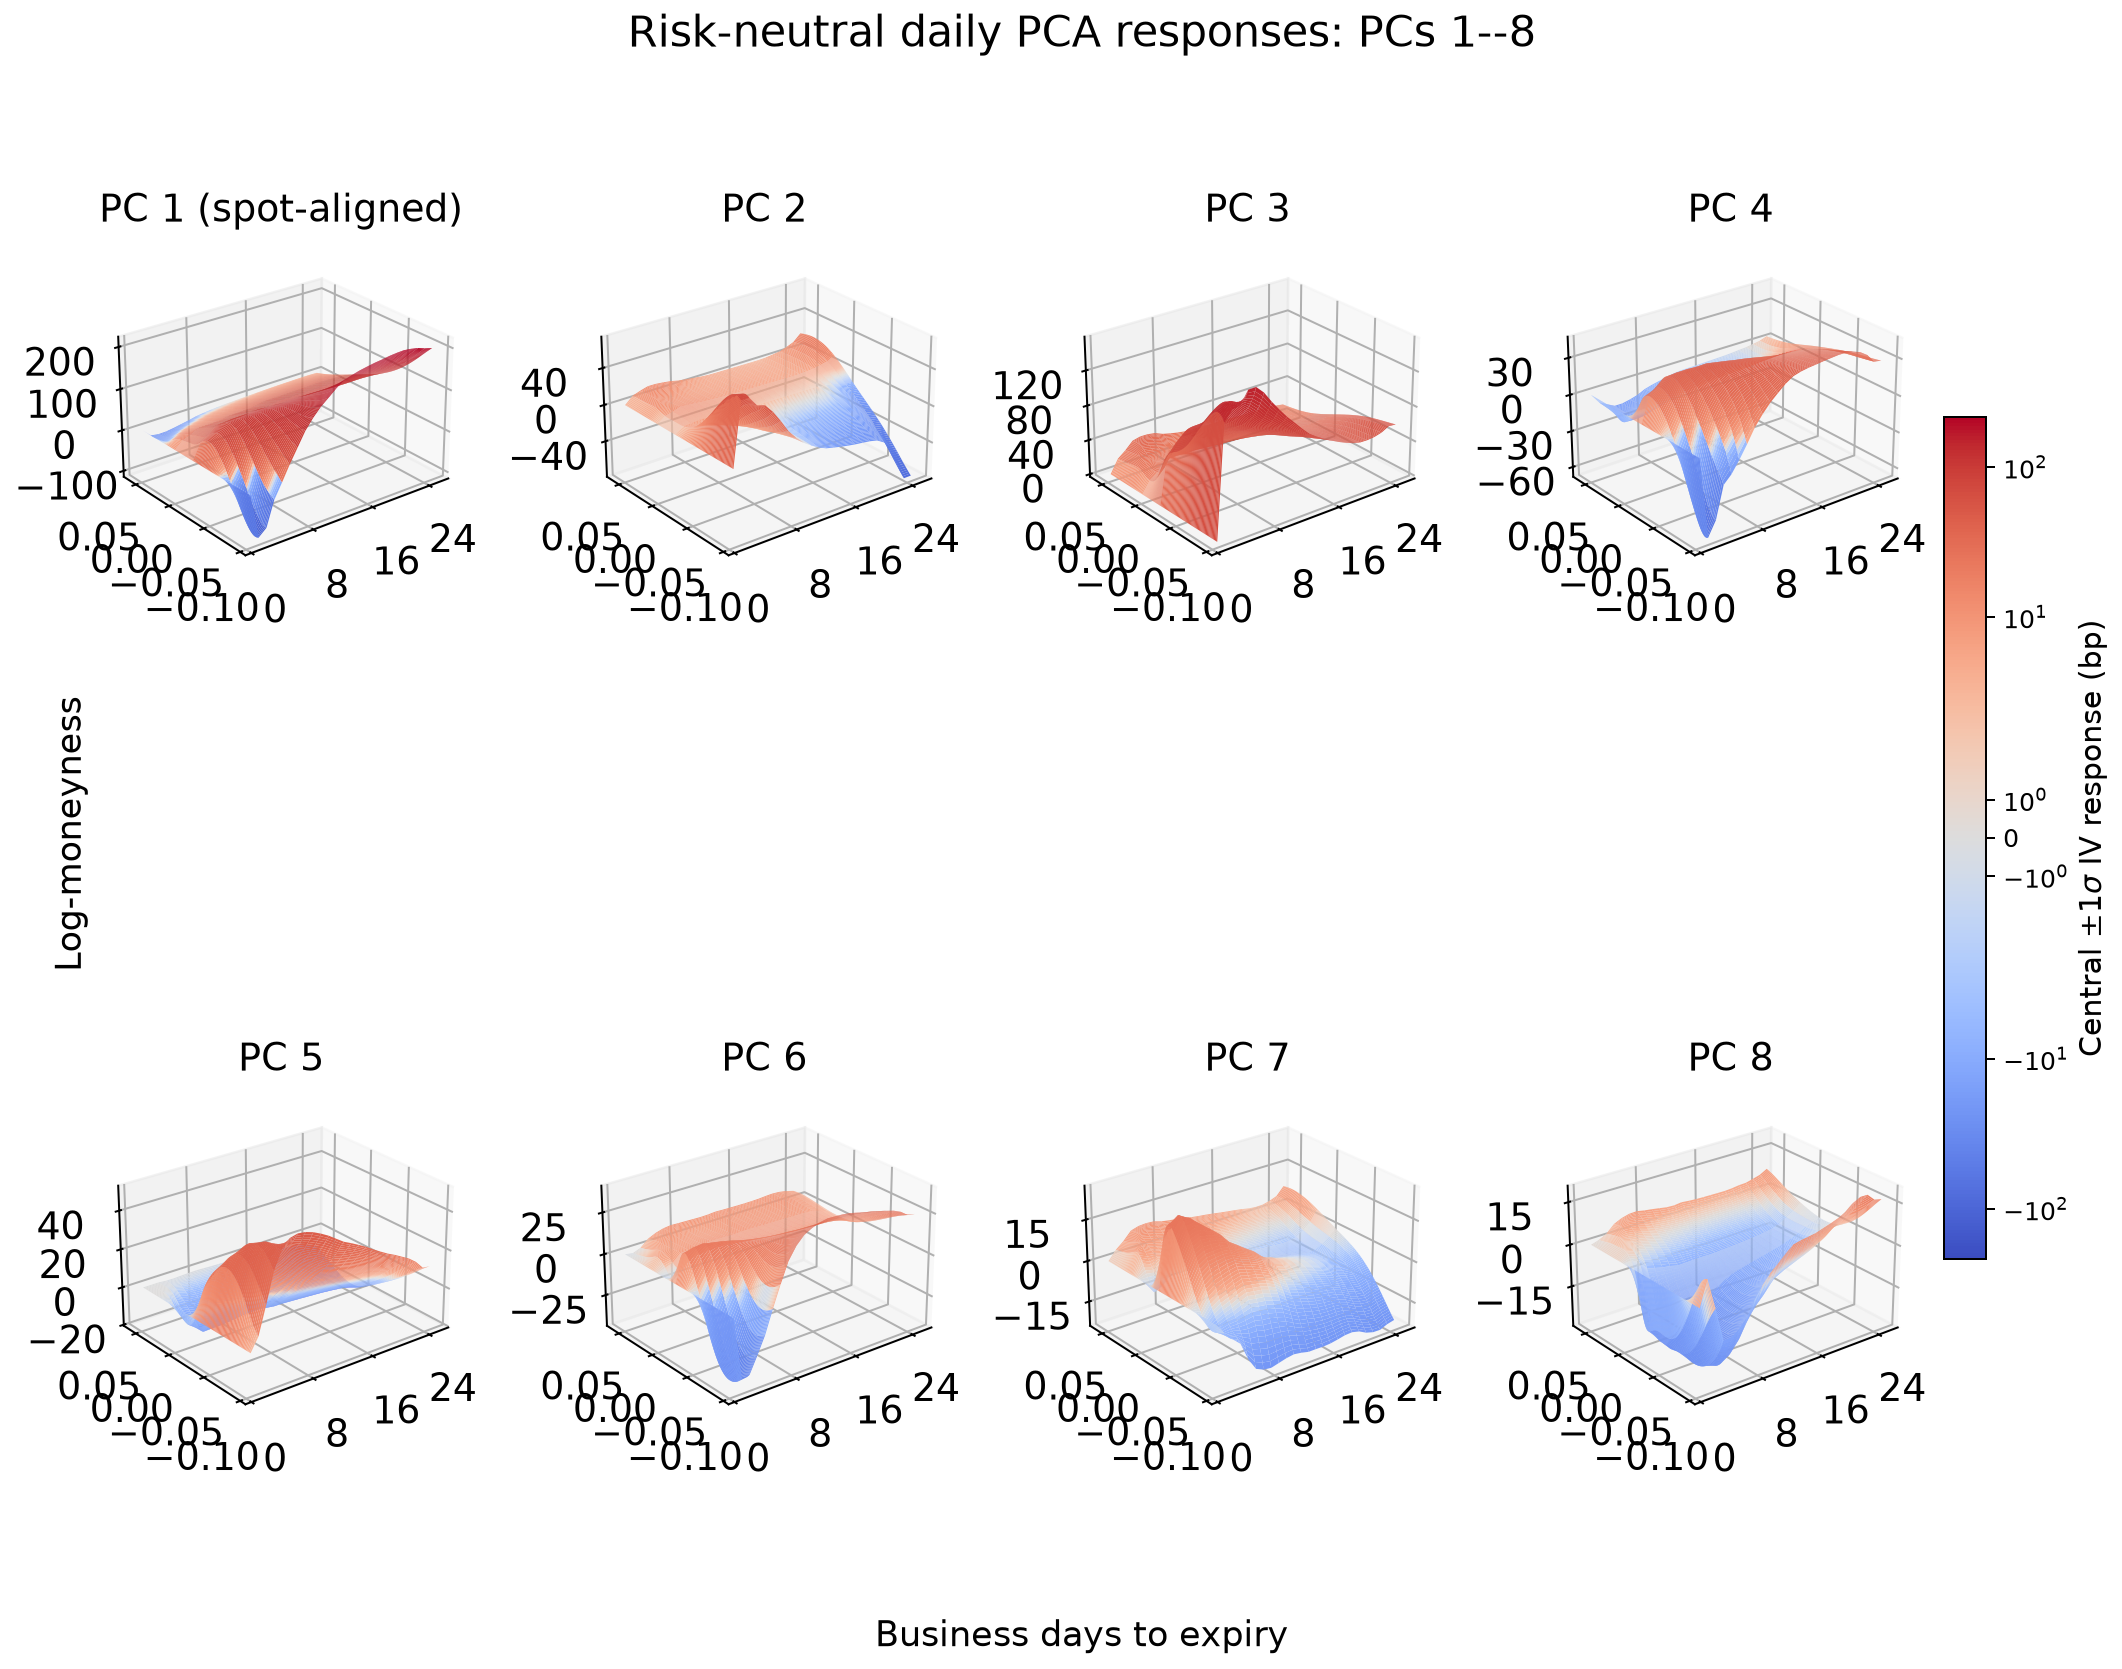
\includegraphics[width=\textwidth]
    {figures/front_spot/pca_factor_responses_3d_pc1_8.png}
  \caption{Risk-neutral one-standard-deviation implied-volatility responses
  for PCs 1--8.  PC~1 is aligned to the front-spot score.}
  \label{fig:numerics-pc1-8}
\end{figure}

\begin{figure}[H]
  \centering
  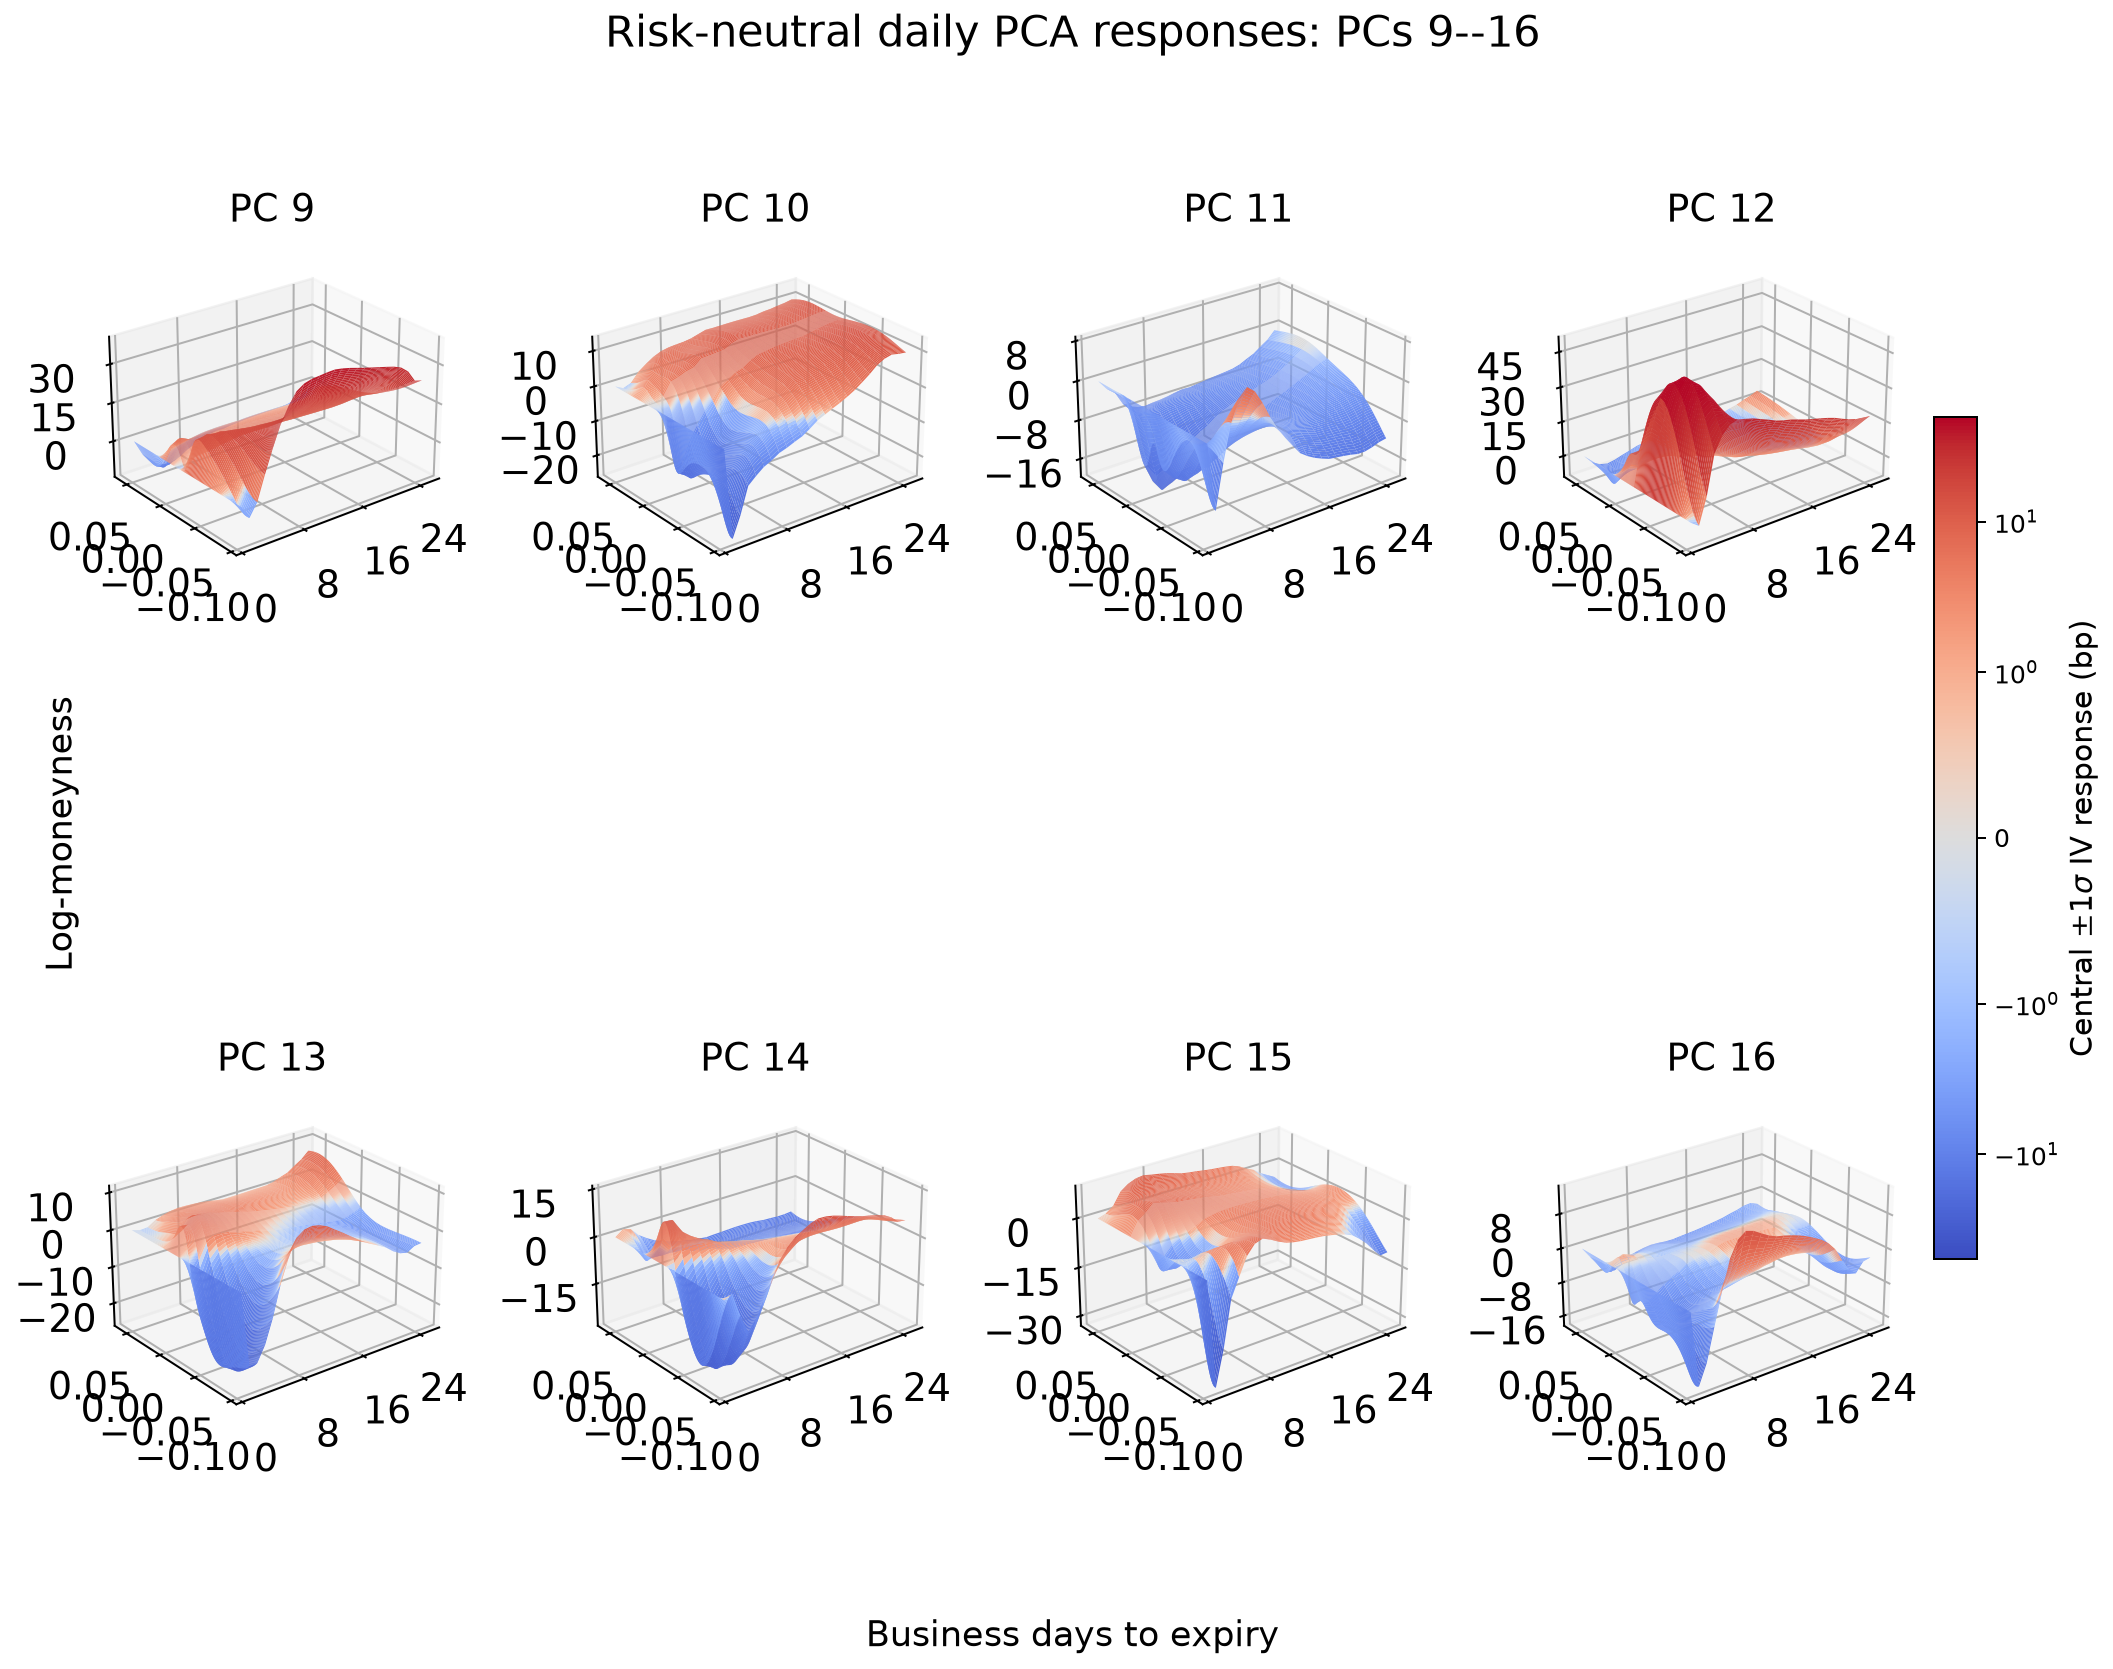
\includegraphics[width=\textwidth]
    {figures/front_spot/pca_factor_responses_3d_pc9_16.png}
  \caption{The additional one-standard-deviation implied-volatility responses,
  PCs 9--16, in the nested rank-16 model.}
  \label{fig:numerics-pc9-16}
\end{figure}
